\documentclass[12pt,a4paper]{scrartcl}
\setlength{\parindent}{0pt}
\setlength{\parskip}{5pt}
\usepackage{times}
\usepackage{theorem}
\usepackage{tikz}
\usepackage{amssymb}
\usetikzlibrary{chains}
\usetikzlibrary{decorations.pathmorphing}
\usepgflibrary{decorations.pathreplacing}
\usetikzlibrary{decorations.text}
\newcommand{\AllReps}{r}
\newcommand{\Indels}{id}
\newcommand{\Size}[1]{|#1}
\theorembodyfont{\rmfamily}
\theoremheaderfont{\rmfamily\bfseries}
\newcounter{Lemmacounter}
\newtheorem{myLemma}[Lemmacounter]{Lemma}
\newcommand{\AfterNumber}{}
\newcommand{\Skiptheorem}{\smallskipamount}
\newcommand{\StartFormal}[1]{\par\addvspace{\Skiptheorem}\noindent\textbf{#1}}
\newcommand{\EndFormal}{\par\addvspace{\Skiptheorem}}
\newenvironment{Lemma}{\begin{myLemma}\AfterNumber}{\end{myLemma}}
\newenvironment{Proof}{\StartFormal{Proof:}}{\EndFormal}
\begin{document}
\def\FirstMultisetSymbol{a} 
\def\SecondMultisetSymbol{b}
\def\ThirdMultisetSymbol{c}
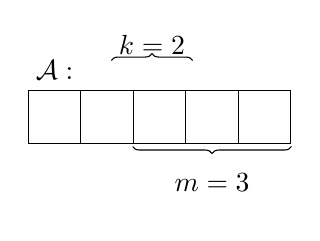
\begin{tikzpicture}
  [arraynode/.style={inner sep=1pt,minimum height=19pt,minimum width=19pt,rectangle,draw},
   alphanode/.style={inner sep=1pt,minimum height=15pt,minimum width=15pt,rectangle},
   position label/.style={
       below = 3pt,
       text height = 1.5ex,
       text depth = 1ex
   },
   overbrace/.style={decoration={brace},decorate},
   underbrace/.style={decoration={brace,mirror},decorate}
   ]
   \begin{scope}[start chain=1 going right,node distance=-0.5mm]
     \node [alphanode,on chain=1] {\(\mathcal{A}:\)};
     \node [alphanode,on chain=1] {\FirstMultisetSymbol};
     \node [alphanode,on chain=1] (A0) {\SecondMultisetSymbol};
     \node [alphanode,on chain=1] (A1) {\ThirdMultisetSymbol};
     \draw [overbrace,decoration={raise=-1ex}] (A0.north west) --
             node [position label,yshift=2.5ex] {\(k=2\)} (A1.north east);
   \end{scope}

   \begin{scope}[shift={(0cm,-17pt)},start chain=2 going right,node distance=-0.15mm]
      \node [arraynode,on chain=2] {\FirstMultisetSymbol};
      \node [arraynode,on chain=2] (Posb) {\FirstMultisetSymbol};
      \node [arraynode,on chain=2] (N0) {};
      \node [arraynode,on chain=2]  {};
      \node [arraynode,on chain=2] (N1) {};
    \draw [underbrace,decoration={raise=1pt}] (N0.south west) --
            node [position label,yshift=-1ex] {\(m=3\)} (N1.south east);
   \end{scope}
\end{tikzpicture}


\begin{Lemma}
\label{Relatesequencelength2editoperations}
Let \(A\) be an alignment of \(u\) and \(v\). Let \(\Indels\) be the number of
insertions and deletions, and \(\AllReps\) be the number of replacements in
\(A\). Then \(\Size{u}+\Size{v}=\Indels+2\cdot\AllReps\).
\begin{Proof}
Each of the \(\Size{u}+\Size{v}\) characters in \(u\) and \(v\) must occur in
\(A\). Moreover, all characters in \(A\) are from the sequences \(u\) and
\(v\). Hence the number of characters in \(A\) and in \(u\) and \(v\) must
be identical. In each indel one character occurs.
In each replacement two of these characters occur. Hence the number of
characters in \(A\) is \(\Indels+2\cdot\AllReps\). By the argumentation above,
this number must be equal to \(\Size{u}+\Size{v}\). So the equation holds.
\(\Box\)
\end{Proof}
\end{Lemma}

\end{document}
